\chapter{Anna - \emph{Identification}}

\section{Proof of concept}
Après avoir pré-traité l'image et trouvé les paragraphes, les lignes et les caractères dans le document, il faut reconnaître ces caractères. Pour ça, nous utilisons un des algorithmes de machine learning les plus répandu: le réseau de neurone feed-forward. Nous allons ici détailler ce que nous avons appris sur cet algorithme, et comment nous l'avons implémenté.

\subsection{Machine learning}

Le machine learning est un champ de recherche dont le but est de trouver des algorithmes capables de s'améliorer sur une tâche particulière avec l'expérience. Souvent, ce que l'on appelle l'expérience consiste en un ensemble d'exemples entrée-sortie correspondant à ce que l'on veut apprendre. Dans notre cas, la tâche du réseau de neurones artificiel sera d'associer à une image de caractère un numéro (par exemple son code ascii), et les exemples sont des paires (image de caractère, numero du caractère).

\subsection{La régression linéaire à une seule variable}

Ramenons nous à un problème plus simple: on a des exemples de la forme $(x, y)$ où $x$ et $y$ sont des nombres, et notre but est de trouver la droite correspondant le mieux à ces exemples.\\
\begin{center}
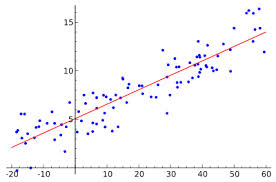
\includegraphics[scale=0.7]{chapters/Pictures/linearregression.jpg}\\
\end{center}
La ligne sera de la forme $h_w(x) = w_1x + w_0$. La première chose à faire est de déterminer une fonction d'erreur pour évaluer les différentes droites possibles. Il se trouve que l'erreur quadratique possède des propriétés intéressantes (comme le fait d'être toujours positive et dérivable). Cette fonction d'erreur s'écrite comme suit :\\
$Err(h_w) = \sum\limits_{j=1}^{N}(y_j - h_w(x_j))^{2}$\\
où $(x_j, y_j)$ est le j-ème exemple et $h_w(x_j)$ est l'image du point $x$ par la droite $h_w : x \rightarrow w_1x + w_0$. Notre but est maintenant de minimiser cette fonction. Imaginons que cette fonction a une forme de bol, et que nous commencions à un point $(w_1, w_0)$ aléatoire de cette fonction (c'est à dire, avec une droite du plan aléatoire). Pour trouver le minimum de cette fonction, il suffit de suivre la pente vers le bas. Mathématiquement parlant, cela signifie qu'il faut prendre le point actuel, et lui soustraire le gradient de la fonction d'erreur. Ce gradient est multiplié par une constante appelée taux d'apprentissage, noté $\alpha$, pour réguler la taille du pas. Un faible taux d'apprentissage signifie une convergence lente, mais avec un taux trop haut, on risque de passer par dessus le minimum et de ne pas converger. On modifie donc le point courant avec la formule :\\

$w_i \leftarrow w_i - \alpha \frac{\partial}{\partial w_i} Err(w)$\\

\subsection{La régression linéaire à plusieurs variables}

L'exstension de cet algorithme à plusieurs variables se fait assez naturellement. Notons $\textbf{x} = (x_0, x_1, \ldots, x_n)$ r. La fonction d'estimation devient alors $h_w(\textbf{x}) = w_nx_n + \cdots + w_1x_1 + w_0x_0$.

\subsection{La regression logistique}

Ce dont nous avons besoin pour reconnaître les caractères est un algorithme de classification. Nous n'avons besoin que de quelques modifications pour faire de l'algorithme précédent un classificateur binaire : nous gardons la fonction d'estimation $h_w(x)$, mais nous passons ensuite le résultat de cette fonction dans une autre fonction dont la sortie se trouve dans $[0;1]$.  La fonction de pas en est une : sa sortie vaut 0 si son entrée est négative, et 1 sinon. Mais cette fonction n'est pas dérivable, et nous verrons plus tard que cela pose problème. On lui préfère donc souvent la fonction logistique (aussi appelée sigmoïde)\\

Son équation est $g(x) = \frac{1}{1 + e^{-x}}$, et sa dérivée est $g(x)(1 - g(x))$. En applicant le même algorithme que pour la régression linéaire, la formule pour mettre à jour le point actuel devient :\\

$w_i \leftarrow w_i + \alpha (y - h_w(\textbf{x}))
h_w(\textbf{x})(1 - h_w(\textbf{x}))x_i$\\
\begin{center}
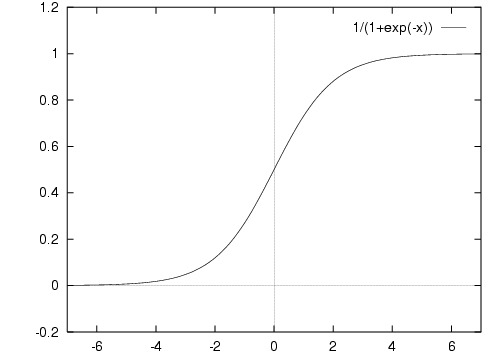
\includegraphics[scale=0.4]{chapters/Pictures/logisticregression.jpg}\\
\end{center}

\subsection{Perceptron}

La régression logistique est la brique de base du réseau de neurones. C'est ce que nous appelons un neurone, du fait de la ressemblance avec le fonctionnement d'un neurone biologique. Maintenant complexifions un peu le problème : nous devons ranger les entrées parmi plusieurs classes possibles. Supposons par exemple que les entrées puissent appartenir à trois classes possibles.\\
La solution est de passer l'entrée à trois neurones différents. Cela produira un vecteur de sortie plutot qu'une simple valeur, et idéalement, ce vecteur convergera vers quelque chose comme (1, 0, 0), (0, 1, 0) ou (0, 0, 1), ces trois vecteurs représentant évidemment les trois classes possibles. Cet algorithme est appelé un réseau de neurones feed-formard à une couche, ou perceptron.\\
\begin{center}
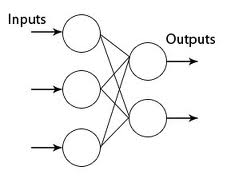
\includegraphics[scale=0.7]{chapters/Pictures/perceptron.jpg}\\
\end{center}

\subsection{Réseau de neurones feed-forward multi-layer}
\subsubsection{Propagation}
Un réseau de neurone feed-forward multi-couches est un perceptron dont le vecteur de sortie sera l'entrée d'un autre percptron, et ansi de suite jusqu'à un perceptron de sortie. Chaque perceptron est appelée une ``couche'' du réseau de neurone. Les couches qui ne sont ni la couche de sortie ni la couche d'entrée sont appelées couches cachées. Le gros avantage d'un réseau de neurones multi-couches par rapport au perceptron est qu'il peu potentiellement calculer n'importe que fonction continue avec seulement une seule couche cachée et avec le bon nombre de neurones dans chaque couche. C'est le résultat énoncé par le théorème universel d'approximation.\\

\begin{center}
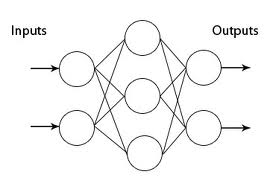
\includegraphics[scale=0.7]{chapters/Pictures/mlffnn.jpg}\\
\end{center}

\subsubsection{Backpropagation}
Pour l'algorithme d'apprentissage, la différence majeure est la fonction dérivée de la fonction d'erreur. Il n'est pas nécessaire ici d'expliciter cette dérivée, mais il est à noter que le calcul de la dérivé des poids d'une couche l dépendra de calculs fait à la couche l+1. Ainsi la mise à jour des poids doit se faire de la dernière couche à la première, d'où le nom de ``backpropagation''.

\subsection{Optimisations}

The only optimization we implemented at this point is the momentum. In the
gradient descent process, we can consider that the current point has some
inertia by adding a certain percentage of the gradient of the last iteration in
the update rule. There are two purposes to this: converging faster, and avoiding
local minimum.

Deux optimisations ont étés implémentées pour augmenter la vitesse de convergence du réseau de neurones et éviter les minimums locaux :
\begin{itemize}
  \item Le moment : appelons $\Delta_n$ le nombre que l'on ajoute à un poids $w_i,j$ à une étape n de l'apprentissage. A l'étape n+1, on ajoutera en plus du gradient de la fonction d'erreur un certain pourcentage de $\Delta_n$. Cela permet à la fois d'éviter les minimums locaux, car le point possède une sorte d'``inertie'', et à la fois de converger plus vite.
  \item Taux d'apprentissage non constant : une technique courante pour augmenter la précision de la convergence est de modifier le taux d'apprentissage au cours du temps. Il est grand au départ pour chercher un minimum global avec peu de précision, puis il diminue pour cherger plus précisément ce minimum.
\end{itemize}

\section{Apprentissage}
L'algorithme décrit dans la section précedente nous a permis de montrer un réseau de neurone apprenant une porte logique quelconque lors de la première soutenance. Pour la deuxième soutenance, la tâche était nettement plus difficile : nous devions être capable de reconnaître une grande quantité de caractères différents et potentiellement de mauvaise qualité.\\
Un problème courant en machine learning, et auquel nous avons étés confrontés, est l'overfitting. On parle d'overfitting quand la fonction que l'on essaye d'apprendre devient trop spécifique aux exemples qu'on lui donne, et qu'elle est incapable de généraliser à d'autres entrées. Etant limités par le temps, nous avons optés pour la solution qui semblait la plus simple à implémenter : entrainer plusieurs réseaux de neurones et classifier en fonction de la moyenne de leur sorties. Nous avons donc essayé avec de plus en plus de réseaux de neurones, jusqu'à ce que les différences deviennent imperceptibles. Nous utilisons donc 20 réseaux de neurones au total.\\
Lors des premiers essais, nous avons aussi eu des problèmes pour trouver la part de responsabilité entre la segmentation et le réseau de neurones. De petites imperfections dans l'un et dans l'autre amène vite à des résultats illisibles.\\
Au jour du rendu, le résultat final est encore loin d'être parfait, de nombreux
caractères sont confondus (9 pour g, c pour e,\ldots ) ou n'ont rien à faire là,
mais nous avons au moins réussi à produire quelque chose malgré les limitations
de temps. \\

